
\documentclass{beamer}
\usepackage{multicol}
\usepackage{braket}
\usepackage{tikzit}
\input{zx-calculus.tikzstyles}
\usepackage{tikz}


\usetheme{metropolis}           % Use metropolis theme
\title{Reconfiguring staggered quantum walks with ZX}
\date{November 5, 2024}
\author{Bruno Jardim \and Jaime Santos \and Luís Soares Barbosa}
\institute{HASLab - INESCTEC}
\begin{document}
\maketitle

\section{Introduction}
\begin{frame}{Introduction}
Optimization of quantum circuits can be seen as a \emph{reconfiguration} process. Indeed the interpretation of such circuits as ZX-diagrams provides a flexible description of quantum computations graphically.
\end{frame}

\section{Introduction to the Staggered Quantum Walk}
\begin{frame}{Staggered Quantum Walk}
	Thought of as the quantum counterpart to classical random walks, quantum walks provide an interesting technique in algorithmic design, with  applications in unstructured search, graph algorithmics and communication protocols.
\end{frame}
\begin{frame}{Staggered Quantum Walk}
	The Staggered Quantum Walks is a recent and very general variant of discrete quantum walks which, avoiding the use of a coin to direct the walker evolution, explores the underlying graph structure to build an evolution operator based on local unitaries induced by adjacent vertices.
\end{frame}

\section{Introduction to the ZX-Calculus}
\begin{frame}{ZX-Calculus}
	The ZX-calculus is diagrammatic language for reasoning about linear maps between qubits and, as such, about quantum computation in general.


\end{frame}

\begin{frame}{ZX-Calculus - Generators}
	\tikzfig{zx-spiders}
\end{frame}
\begin{frame}{ZX-Calculus - Rewrite Rules}



	\begin{multicols}{2}
		\begin{itemize}
			\item Spider Fusion
			      \resizebox{0.4\textwidth}{!}{% 
				      \tikzfig{rule-sf}
			      }%
			\item Identity Removal
			      \resizebox{0.4\textwidth}{!}{% 
				      \tikzfig{rule-id}
			      }%
			\item Color Change
			      \resizebox{0.4\textwidth}{!}{% 
				      \tikzfig{rule-colour-change}
			      }%
			\item Hadamard Identity
			      \resizebox{0.4\textwidth}{!}{% 
				      \tikzfig{rule-had-id}
			      }%
			\item Bialgebra
			      \resizebox{0.4\textwidth}{!}{% 
				      \tikzfig{rule-bialg}
			      }%
			\item $\pi$-commutation
			      \resizebox{0.4\textwidth}{!}{% 
				      \tikzfig{rule-pi-com}
			      }%
			\item Hopf
			      \resizebox{0.4\textwidth}{!}{% 
				      \tikzfig{rule-hopf}
			      }%
			\item State copy
			      \resizebox{0.4\textwidth}{!}{% 
				      \tikzfig{rule-state-copy}
			      }%


		\end{itemize}
	\end{multicols}



\end{frame}
\section{Bringing ZX into the picture}

\begin{frame}{Staggerd Quantum Walk - Circuit}
	A general implementation of a Staggered Quantum Walk for a line graph.

	\ctikzfig{sqw-circuit}

\end{frame}


\begin{frame}{Staggerd Quantum Walk - ZX-diagram}
	A concrete implementation of a Staggered Quantum Walk for a line graph with 3 qubits and the state $\ket{4}$ as the initial state.

	\ctikzfig{1-step-sqw}

\end{frame}
\begin{frame}{Staggerd Quantum Walk - ZX-diagram}
	The previous diagram utilizes a notation from the ZH-calculus for the Tofolli gates that greatly simplifies the diagram. Expanding the Tofolli gates it yields
	\begin{align*}
		\resizebox{0.9\textwidth}{!}{% 
			\tikzfig{1-step-expanded}
		}%
	\end{align*}
\end{frame}
\begin{frame}{Staggerd Quantum Walk - ZX-diagram}
	\begin{align*}
		\resizebox{0.9\textwidth}{!}{% 
			\tikzfig{1-step-trivial}
		}%
	\end{align*}
\end{frame}

\begin{frame}{Staggerd Quantum Walk - ZX-diagram}
	Unfortunately this is the limit one can reasonably optimize the circuit by hand.

	This is where PyZX comes in.
\end{frame}

\section{PyZX}
\begin{frame}{Automated Diagrammatic Rewriting - PyZX}
	PyZX is a Python tool implementing the theory of ZX-calculus for the creation, visualization, and automated rewriting of large-scale quantum circuits.
\end{frame}

\begin{frame}{Automated Diagrammatic Rewriting - PyZX}
	Advanced techniques directly implemented in PyZX as the \texttt{full\_reduce} method, may reduce the circuit T-count in about $50\%$.
	
	However, the resulting diagram no longer resembles a circuit, making direct comparisons with the original one difficult.
\end{frame}

\begin{frame}{Staggered Quantum Walk - Graph-like}
	
	\begin{align*}
		\resizebox{0.9\textwidth}{!}{% 
			\tikzfig{graph-like}
		}%
	\end{align*}
\end{frame}

\begin{frame}{Optimization Comparison - Total Number of Gates}
	
	\begin{table}[H]
		
		\centering
		\resizebox{\textwidth}{!}{\begin{tabular}{|l|cccc|}
			
		\hline
									   & \multicolumn{4}{l|}{Number of steps in the staggered quantum walk:}                                   \\ \hline
		Optimizations used:          & \multicolumn{1}{c|}{1}  & \multicolumn{1}{c|}{2}  & \multicolumn{1}{c|}{4}   & 8   \\ \hline
		None            & \multicolumn{1}{c|}{39} & \multicolumn{1}{c|}{77} & \multicolumn{1}{c|}{153} & 305 \\ \hline
		Simple     & \multicolumn{1}{c|}{31} & \multicolumn{1}{c|}{59} & \multicolumn{1}{c|}{115} & 227 \\ \hline
		Full-reduce + fusion/id/to\_rg & \multicolumn{1}{c|}{37} & \multicolumn{1}{c|}{47} & \multicolumn{1}{c|}{72}  & 118 \\ \hline
	
		\end{tabular}
		}
		%\label{tab:total-gates}
		\end{table}
		
\end{frame}	
\begin{frame}{Optimization Comparison - T-count}	
	\begin{table}[H]
		\centering
		\resizebox{\textwidth}{!}{\begin{tabular}{|l|cccc|}
		\hline
									   & \multicolumn{4}{l|}{Number of steps in the staggered quantum walk:}                                  \\ \hline
		Optimizations used:          & \multicolumn{1}{c|}{1}  & \multicolumn{1}{c|}{2}  & \multicolumn{1}{c|}{4}  & 8   \\ \hline
		None            & \multicolumn{1}{c|}{16} & \multicolumn{1}{c|}{32} & \multicolumn{1}{c|}{64} & 128 \\ \hline
		Simple       & \multicolumn{1}{c|}{16} & \multicolumn{1}{c|}{32} & \multicolumn{1}{c|}{64} & 128 \\ \hline
		Full-reduce + fusion/id/to\_rg & \multicolumn{1}{c|}{10} & \multicolumn{1}{c|}{16} & \multicolumn{1}{c|}{28} & 52  \\ \hline
		\end{tabular}}
		\end{table}
		
\end{frame}

\section{An alternative evolution operator}
\begin{frame}{An alternative evolution operator}	
When analyzing the  ZX diagram for a long staggered quantum walk (i.e. with more than 5 steps)  a pattern starts to emerge, repeating itself as many times as  the number of steps considered.
\end{frame}

\begin{frame}{An alternative evolution operator}	
	\begin{align*}
		\tikzfig{sqw-pattern-standard}
	\end{align*}
	where $\alpha_n = \pm \frac{\pi}{4}$ and $\beta_n = \frac{2\pi}{3} + m\pi$, with $m=0$ or $m=1$.
\end{frame}

\begin{frame}{An alternative evolution operator - Generalization}	
	\begin{align*}
		\resizebox{0.9\textwidth}{!}{
		\tikzfig{sqw-pattern-generalization}
		}
	\end{align*}
\end{frame}
\begin{frame}{An alternative evolution operator - Rationale}	
The rationale behind this operator is easy to explain: it creates a uniform distribution over a certain number of states, applies a rotation that makes some states more likely than others and then spreads these probabilities over the remaining states using CNOT gates. This also explains why the pattern only shows up in staggered quantum walks over a certain length. 
\end{frame}
\begin{frame}{An alternative evolution operator - Advantages}	
	\begin{itemize}
		\item Reduces the total amount of gates needed to represent the evolution of the quantum walk
		\item Only uses gates controlled by at most 1 qubit
		\item To go from an $n$-qubit to an $n+1$ qubit quantum walk, all that needs to be done is to add two more XCX-gates
	\end{itemize}
\end{frame}
\begin{frame}{An alternative evolution operator - Advantages}	
	In general, this makes the alternative operator much more efficient with respect to the total number of gates used, leading to lower depth  and, therefore, potentially less error-prone circuits.
\end{frame}

\begin{frame}{An alternative evolution operator - Disadvantages}	
However, a number of challenges remain, requiring further investigation. These concern the most suitable choice of parameters for $\alpha_n$ and $\beta_n$, as well as whether and how they depend on the number of qubits used in a particular staggered walk. 
\end{frame}
\begin{frame}{An alternative evolution operator - Example}	
	\begin{align*}
		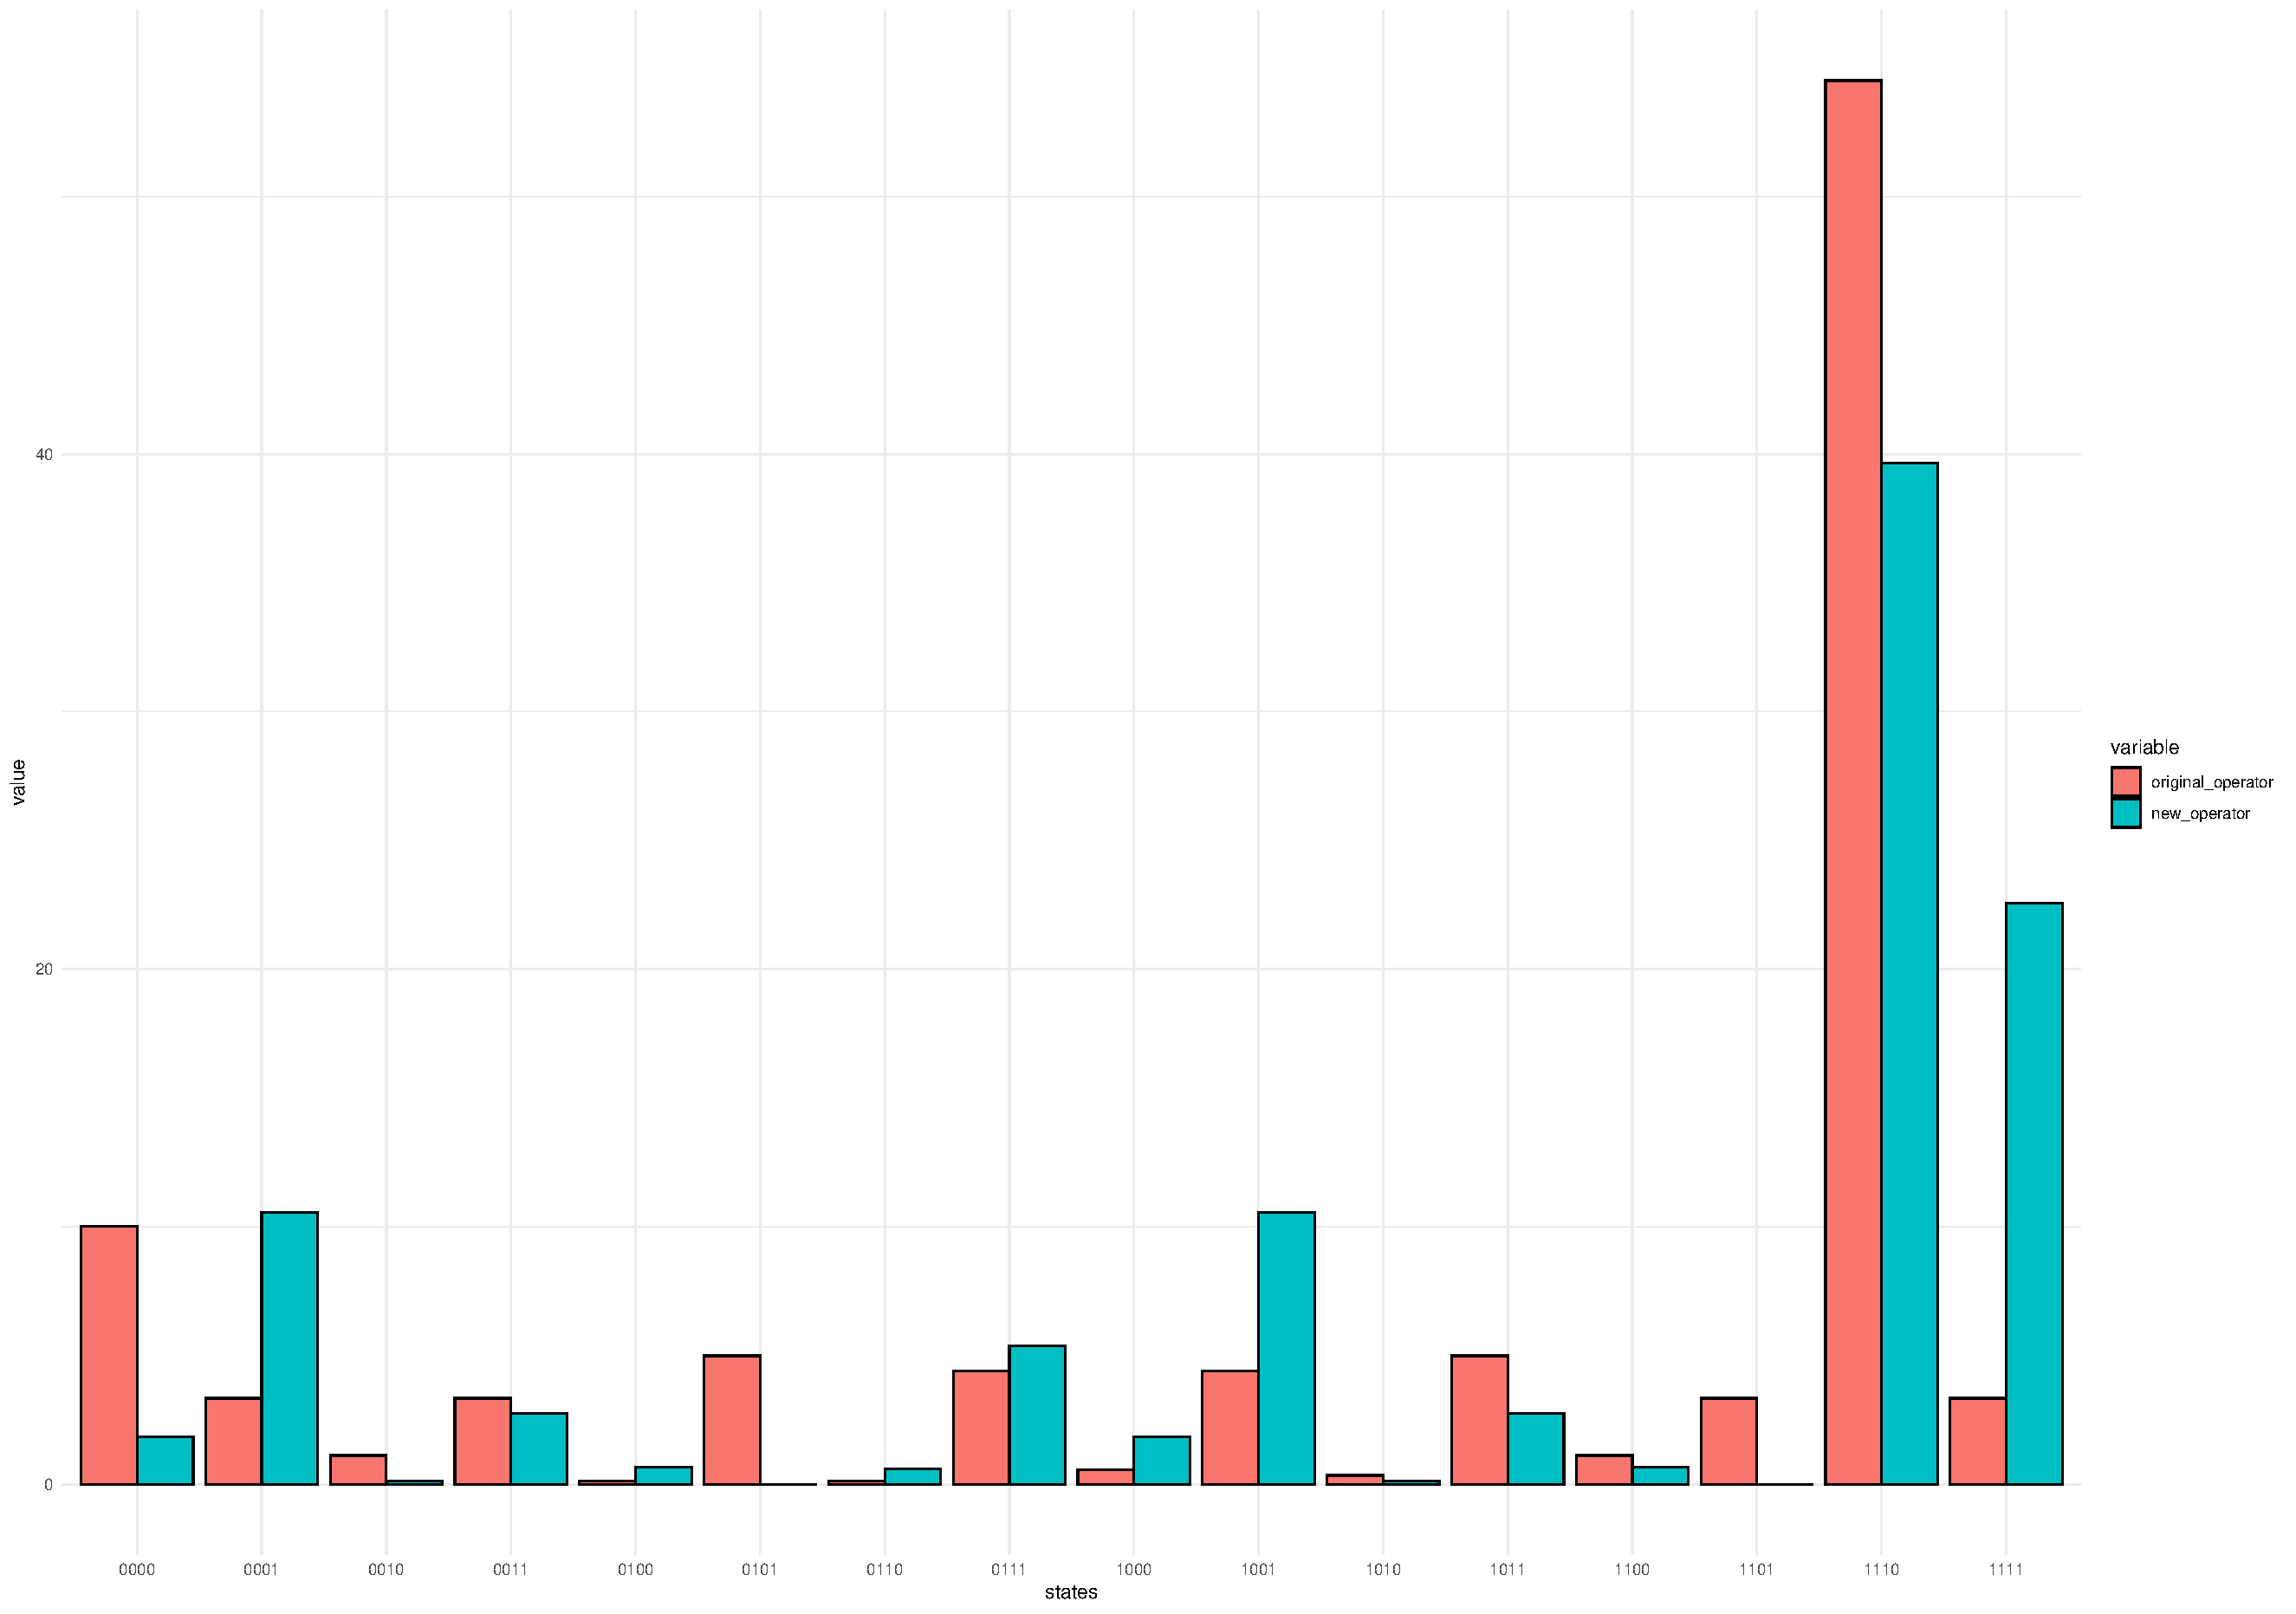
\includegraphics[width=0.9\linewidth]{figures/new_4step.pdf}
	\end{align*}
\end{frame}

\section{Conclusions and future work}
\begin{frame}{Conclusions}	
	The original, 'intuitive' implementation of a staggered quantum walk can be heavily optimized with respect to both the total number of gates and the T-count value.
	
	It also lead to the identification of an alternative formulation of the evolution operator with a significant reduction in the number of gates involved and thus suitable for running on more limited quantum processing units.
	
\end{frame}
\begin{frame}{Conclusions - (cont.)}	
	This exercise regards algorithmic optimisation  in quantum programming  as a \emph{graph reconfiguration} process. This has a huge potential in the development of hybrid quantum-classical algorithms, which are the ones that can actually run in current quantum devices.
	
	They are essentially dynamic in the sense that, depending on a measurement carried over the quantum state, the quantum code running in the quantum device acting as a co-processor is transformed on-the-fly.
\end{frame}
\end{document}
